\documentclass[12pt]{article}

%%    LES PACKAGES
\usepackage{import}
\usepackage{enumitem}%Pour faire des listes à puces stylés.
\usepackage{pifont} %Pour changer les symboles dans les listes à puces.
\usepackage{stmaryrd}%Pour les intervalles discrets.
\usepackage{amsmath}
\usepackage{amsfonts}
\usepackage{amssymb}
\usepackage{amsthm}
\usepackage{esint}
\usepackage[most,many,breakable]{tcolorbox}
\usepackage{graphicx}
\usepackage{color}
\usepackage{nicefrac}
\usepackage{mathtools}
\usepackage{xcolor}
\usepackage{awesomebox}
\usepackage{cancel}
\usepackage{setspace}
\usepackage{varwidth}
\usepackage{mathrsfs}
\usepackage[frenchb]{babel}
\usepackage[left=1cm, right=1cm, top=2cm, bottom=2cm]{geometry}

%%    MISE EN PAGE





\definecolor{Aquamarine}{HTML}{00B5BE}
\DeclareMathSizes{10}{9}{7}{5}
\baselineskip=12pt


%%%%%%%%%%%%%%%%%%%%%%%%%%%%%%
%%    LES ENVIRONNEMENTS
%%%%%%%%%%%%%%%%%%%%%%%%%%%%%%


\newtheorem{definition}{Définition}[section]
\newtheorem{propriete}{Propriétés}
\newtheorem{theoreme}{Théorème}
\newtheorem*{proposition}{Proposition}
\newtheorem*{preuve}{Preuve}
\newtheorem*{remark}{Remarque}
\newtheorem{exercice}{Exercice}
\newcommand{\defi}{\begin{tcolorbox}[title=Définition, colframe=red!75!black, colback=red!10!white]}
\newcommand{\prop}{\begin{tcolorbox}[title=Propriété, colframe=blue!85!black, colback=blue!10!white]}
\newcommand{\impo}{\begin{tcolorbox}[title=Points importants, colframe=black!0!black, colback=black!0!white]}
\newcommand{\close}{\end{tcolorbox}}
\newtcolorbox{mybox}{colback=black!5!white,colframe=black!75!black}


%% LES MACROS
\newcommand{\summ}[2]{\sum_{#1}^{#2}}
\newcommand{\dps}{\displaystyle}
\newcommand{\sk}{\smallskip}
\newcommand{\bk}{\bigskip}
\newcommand{\jump}{~~}
\newcommand{\acc}[1]{\hspace{-0.05cm}\left\{#1 \right\}}
\newcommand{\parr}[1]{\hspace{-0.05cm}\left(#1 \right)}
\newcommand{\rect}[1]{\left[ #1 \right]}
\newcommand{\braks}[1]{\hspace{-0.05cm}\llbracket#1 \rrbracket}
\newcommand{\abs}[1]{\hspace{-0.05cm}\left\lvert#1 \right\rvert}
\newcommand{\eq}{\Leftrightarrow}
\newcommand{\mc}[1]{\mathcal{#1}}
\newcommand{\mb}[1]{\mathbb{#1}}
\newcommand{\mr}[1]{\mathscr{#1}}
\newcommand{\Ra}{\Rightarrow}
\newcommand{\projet}[3]{p_{#1\Vert #2}(#3)}
\newcommand{\projeet}[2]{p_{#1\Vert #2}}
\newcommand{\ra}{\rightarrow}
\newcommand{\lra}{\longrightarrow}
\newcommand{\la}{\leftarrow}
\newcommand{\exs}{\exists}
\newcommand{\fonction}[3]{#1:#2\longrightarrow#3}
\newcommand{\famille}[3]{#1_#2,\dots,#1_#3}
\newcommand{\transpose}[1]{{}^{t\!}#1}
\newcommand{\longvec}[1]{\overrightarrow{#1}}

%% MACRO POUR LES MBOX
\newcommand{\tw}{\textwidth}
\newcommand{\blue}{\color{blue}}
\newcommand{\red}{\color{red}}
\newcommand{\green}{\color{green}}






\title{Projet MAM3 : Régression linéaire}
\author{Ben Khalifa Emna, Costantin Perline, Honakoko Giovanni}
\date{26/05/2025}

	\setlength{\intextsep}{12pt plus 2pt minus 2pt} % Espace autour des figures
\setlength{\textfloatsep}{12pt plus 2pt minus 2pt} % Espace entre figures
\setlength{\parindent}{0pt} % Supprime l'indentation de tous les paragraphes


\begin{document}
	\maketitle
	
	\vspace{2cm}
	
\begin{figure}[hbtp]
	\centering
	\noindent
	
	\begin{minipage}[t]{0.35\textwidth}
		\vspace{0pt} % force l'alignement en haut
		\small
		La régression linéaire est un type de modélisation mathématique permettant de faire des prédictions \textit{(droite rouge)} à partir d’un jeu de données \textit{(nuage de points)} réelles.
	\end{minipage}
	\hfill
	\begin{minipage}[t]{0.6\textwidth}
		\vspace{0pt} % force l'alignement en haut
		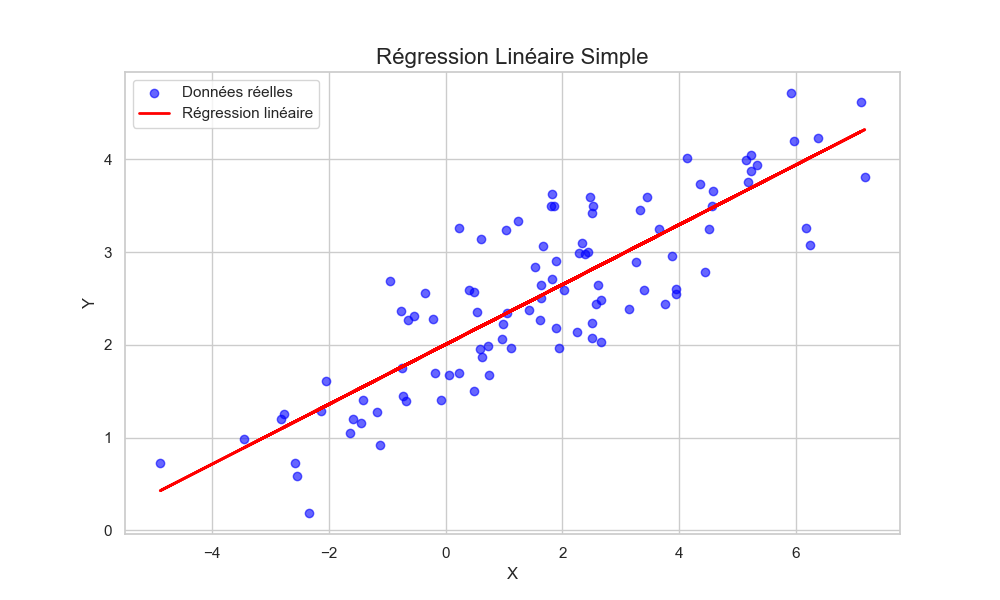
\includegraphics[width=\linewidth]{img/regress_simple1.png}
	\end{minipage}%

\end{figure}
	
	
	
	\newpage
	\tableofcontents
	
	\section{Modèle de régression linéaire simple}
	\subsection{Cadre}
	On se place dans le cadre de la régression linéaire simple où on a une variable réponse et une variable explicative qui sont quantitatives.
	On dispose de $\mc{L} := \acc{(x_{i},y_{i})_{i \in \braks{1,n}}}$ où :
	\begin{itemize}[label*=\textbullet]
		\item $i$ représente l'individu considéré 
		\item $x_{i}$ représente les observations de la variable explicative
		\item $y_{i}$ représente les observations de la variable réponse
	\end{itemize}
	On cherche $f$ la fonction telle que : $\forall i \in \braks{1,n}, y_i \approx f(x_i)$. Afin d'estimer $f$, on veut minimiser une quantité que l'on appelle risque quadratique : 
	\begin{equation*}
		R(\tilde{f}) := \mb{E}\rect{\parr{Y- \tilde{f}(X)}^{2}}
	\end{equation*}
	où $Y$ est la variable réponse et $X$ est la variable explicative. La quantité $R$ mesure l'erreur quadratique moyenne entre les valeurs observées et les valeurs prédites.
	

	Cette quantité étant purement théorique, voir quasiment inaccessible en réalité,  on l'a substitue à son équivalent empirique: 
	\begin{equation*}
		R_{n}(\tilde{f}) := \dfrac{1}{n}\sum_{i=0}^{n}\parr{Y_{i} -\tilde{f}(X_i)}^{2}
	\end{equation*}
	
	Comme nous l'avons vu dans la vulgarisation en première page, on souhaite que nos prédictions suivent une droite affine. 
	Donc on restreindra $\tilde{f}$ à l'ensemble $\mc{F} = \acc{g : \mb{R}\lra \mb{R} , \hspace{2mm} g(x)= ax + b, \forall a,b \in \mathbb{R}}$.
	
	Dans notre cadre $Y_{i} = ax_{i}+ b + \varepsilon_{i}$ où $\varepsilon_i$ représente le bruit pour l'individu $i$.
	
	Les $Y_{i}$ et les $\varepsilon_{i}$ sont des quantités aléatoires contrairement aux $x_{i}$ qui sont fixes.
	\bk 
	
	
	On se ramène à un problème de moindres carrés où nous voulons minimiser la distance qu'il y a entre nos points et l'espace affine engendré par $\tilde{f}$, c'est à dire minimiser $\sum_{i=1}^{n}x_i \parr{Y_i - \tilde{f}(x_i)}^{2}=\sum_{i=1}^{n}x_i \parr{Y_i - ax_{i} - b}^{2}$.
	
	\subsection{Estimation paramétrique}
	On pose : 
	\begin{equation*}
		\overline{x}_{n} = \frac{1}{n}\sum_{i=1}^{n}x_i\quad , \quad  \overline{Y}_{n} = \frac{1}{n}\sum_{i=1}^{n}Y_i
	\end{equation*}
	On cherche les points critiques : 
	\begin{align*}
		&\begin{cases}
			\dps 
			\frac{\partial R_{n}(g)}{\partial a} = 0
			\\
			\dps \frac{\partial R_{n}(g)}{\partial b} = 0
		\end{cases}
		\\
		&\begin{cases}
			\dps 
			-\frac{2}{n}\sum_{i=1}^{n}x_i \parr{Y_i - ax_i - b } = 0
			\\
			\dps -\frac{2}{n}\sum_{i=1}^{n}(Y_i - ax_i - b) = 0
		\end{cases}
		\\
		&\begin{cases}
			\dps 
			\sum_{i=1}^{n} x_i Y_i - a\sum_{i=1}^{n}x_i^{2} - b\sum_{i=1}^{n}x_i = 0
			\\
			\dps b = \overline{Y}_{n} - a\overline{b}_n
		\end{cases}
	\end{align*}
	
	En réinjectant l'expression de $b$ dans la première ligne on obtient :
	\begin{align*}
		\sum_{}^{}x_iY_i - \overline{Y}_n\sum_{i=1}^{n}x_i - a\overline{x}_n\sum_{i=1}^{n}x_i &= 0
		\\
		\sum_{i=1}^{n}x_i Y_i - \overline{Y}_{n} \sum_{i=1}^{n}x_i &= a \rect{ \sum_{i=1}^{n}x_i^{2} - \overline{x}_n \sum_{i=1}^{n}x_i }
		\\
		\sum_{i=1}^{n}x_i Y_i -n\overline{y}_n \overline{x}_n&= a \rect{\sum_{i=1}^{n}x_i^2 -n\parr{\overline{x}_n}^2} 
		\\
		a&=\dfrac{\sum_{i=1}^{n}x_i Y_i -n\overline{Y}_n \overline{x}_n}{\sum_{i=1}^{n}x_i^2 -n\parr{\overline{x}_n}^2}
	\end{align*}
Ainsi on pose :
\begin{equation*}
	\begin{cases}
		\hat{a}_{n}=\dfrac{\sum_{i=1}^{n}x_iY_i -n\overline{Y}_n \overline{x}_n}{\sum_{i=1}^{n}x_i^2 -n\parr{\overline{x}_n}^2}
		\\
		\hat{b}_{n}=\overline{Y}_n - a\overline{x}_{n}
	\end{cases}
\end{equation*}
\ding{110}

\subsection*{Proposition}
Les estimateurs $\hat{a}_{n}$ et $\hat{b}_{n}$ sont sans biais.

\textsc{Preuve}

\ding{110}

\subsection{Propriétés des estimateurs $\hat{a}_{n}$ et $\hat{b}_{n}$}
Pour nos estimateurs $\hat{a}_{n}$ et $\hat{b}_{n}$ on a :
\begin{itemize}[label*=\textbullet]
	\item $\mb{V}\rect{\hat{b}_{n}} = \dfrac{\sigma^{2} \sum_{i=1}^{n} x_i^2}{n\sum_{i=1}^{n}(x_{i} - \overline{x}_{n})^2 }$ et $\mb{V}\rect{\hat{a}_n} = \dfrac{\sigma^2}{\sum_{i=1}^{n} (x_i - \overline{x}_{n})^2}$
	\item $\mathrm{cov}(\hat{a}_{n},\hat{b}_{n}) = \dfrac{-\sigma^{2}\overline{x}_{n}}{\sum_{i=1}^{n} (x_i - \overline{x}_{n})^2}$
\end{itemize}

\textsc{Preuve}


\ding{110}

Or on ne connaît pas non plus la valeur de $\sigma^2$ ce qui nous pousse à utiliser un estimateur d'un tel paramètre.

Un estimateur sans biais de cette quantité est $\dps \hat{\sigma}^{2}_{n} = \dfrac{1}{n-2}\sum_{i=1}^{n}\parr{Y_{i} - \hat{Y}_{i}}^2$, avec $\hat{Y}_{i} = \hat{a}_{n}x_i + \hat{b}_{n}$ la prédiction des $Y_{i}$ par le modèle de régression linéaire.

\subsection{Validité de la régression linéaire}
On appelle coefficient de détermination $R^{2}$ la quantité définie par : 
\begin{equation*}
	R^{2} = \dfrac{\sum_{i=1}^{n} \parr{\hat{Y}_i - \overline{Y}_{n} }^{2} }{\sum_{i=1}^{n}\parr{Y_i - \overline{Y}_{n}}^{2} } = 1 - \dfrac{\sum_{i=1}^{n} \parr{\hat{Y}_{i} - Yi}^{2} }{\sum_{i=1}^{n}\parr{Y_i - \overline{Y}_{n}}^{2}} = \parr{\mathrm{corr}\parr{Y_i,\hat{Y}_i}}^{2}
\end{equation*}
Ainsi définit cette quantité mesure la variance des résidus par rapport à la variance notre jeu de donnée et ainsi relate de la dispersion des observations par rapport à la droite de régression.


La validation de notre modèle de régression linéaire est déterminée par les conditions:
\begin{itemize}[label*=\textbullet]
	\item $R^2 \in \rect{0,1}$
	\item Test paramétrique sur $\boldsymbol{a}$ concluant sur $\mc{H}_{1}$
\end{itemize}

Plus $R^2$ sera proche de $1$, plus notre modélisation sera juste. Cependant il est important de pouvoir supposer la normalité du bruit en amont de ces vérifications. De plus cette hypothèse n'est pas vérifiée pour le coefficient de détermination :



\section{Modèle de régression linéaire multiple}

\section{Analyse de la variance}


\end{document}